\section{Introduction}
\begin{frame}
\frametitle{Présentation du sujet}
\begin{center}
\begin{itemize}
\item Programmation sur un drone
\item Réalisation d'un jeu mobile
\item Architecture client-serveur
\end{itemize}
\begin{figure}
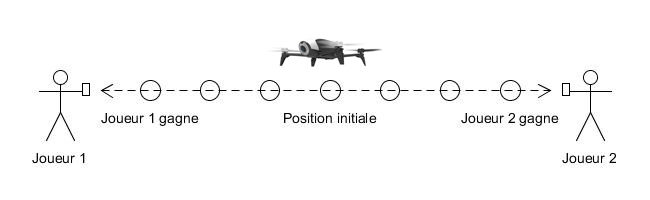
\includegraphics[scale=0.4]{images/partie.jpg}
\end{figure}
\end{center}

\textbf{BUT :} Contrôle à distance du drone

$\implies$ Démonstration publique à la \textit{Fête de la Science}
\end{frame}

\begin{frame}
\frametitle{Les outils}
\begin{minipage}[t]{.46\linewidth}
      \begin{center}
      DRONE PARROT BEBOP 2
      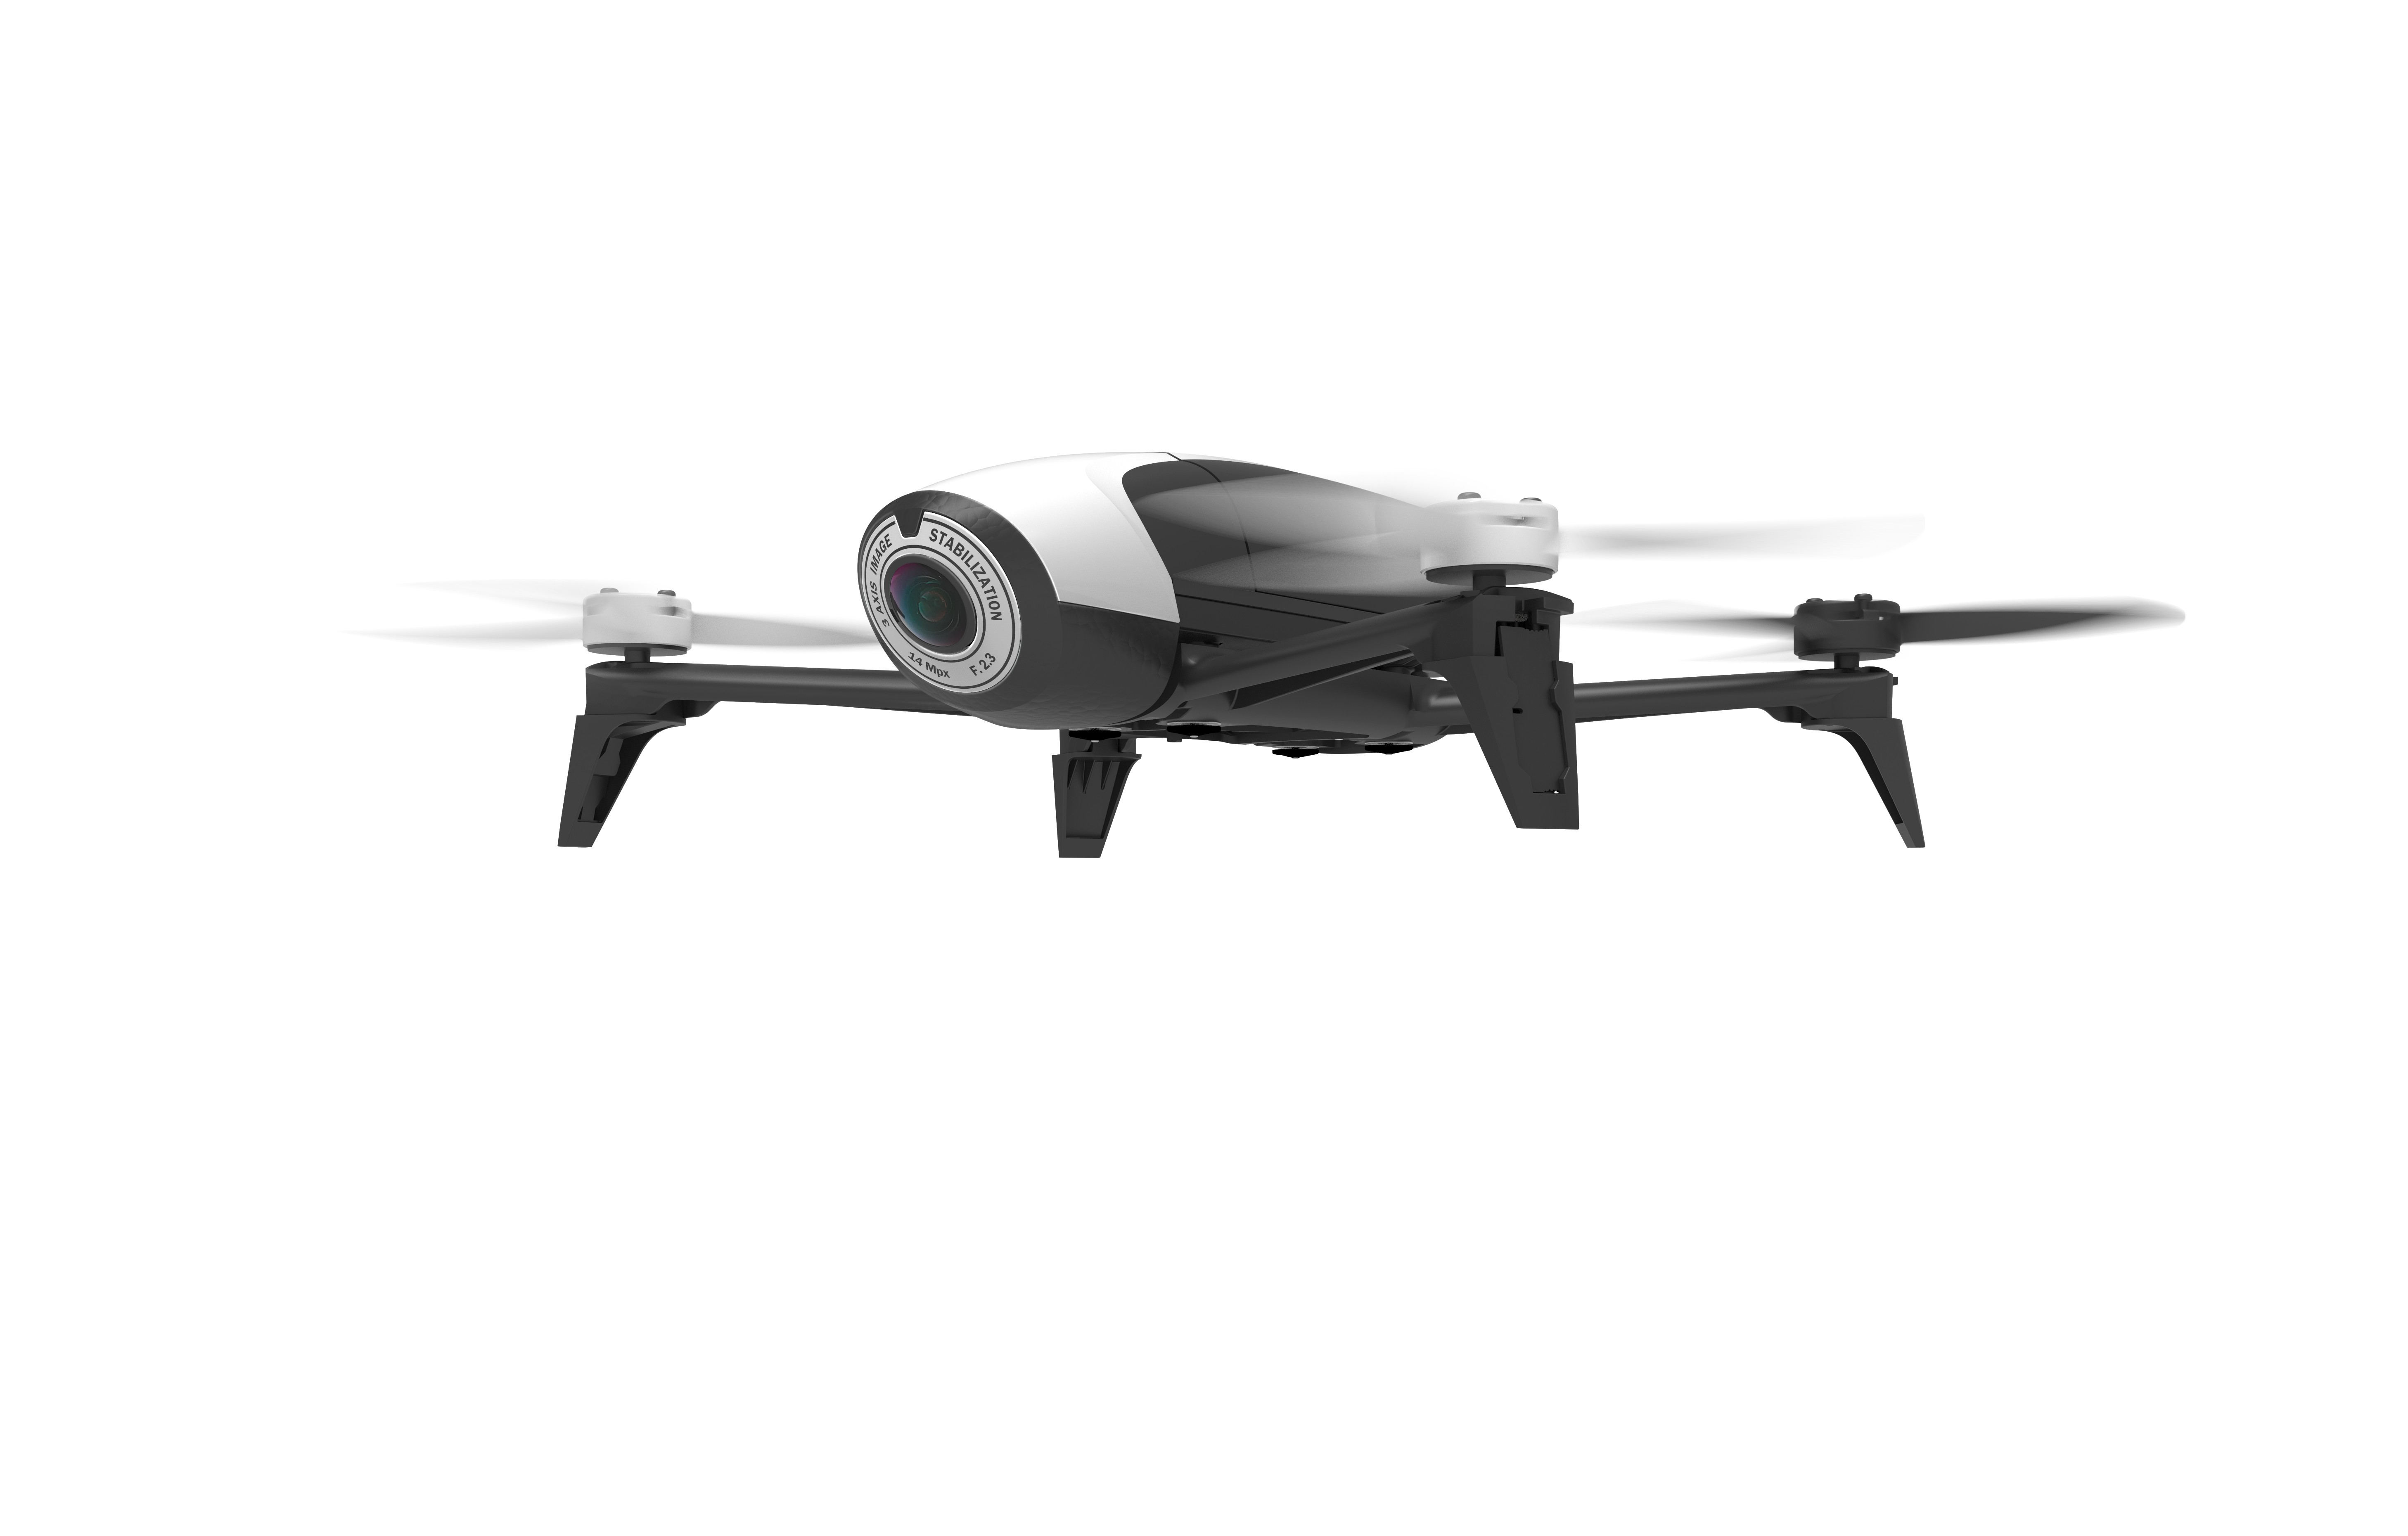
\includegraphics[scale=0.02]{images/drone.jpg}
      \begin{itemize}
      \item Poids : 500g
      \item Autonomie : 25min
      \item Diffuse un réseau Wi-Fi sur 300m
      \item Application mobile \textit{Free Flight Pro}
      \end{itemize}
      \end{center}
   \end{minipage} \hfill
   \begin{minipage}[t]{.46\linewidth}
      \begin{center}
      ANDROID SDK
      
\includegraphics[scale=0.2]{images/android.jpg}
      \begin{itemize}
      \item Java
      \item Framework \textit{libGDX}
      \end{itemize}
      \end{center}
   \end{minipage}
\end{frame}